\documentclass[landscape]{article}
%\usepackage[top=0.4in,bottom=0.4in,left=0.75in,right=0.5in]{geometry}
\usepackage[paperwidth=13.13636in,paperheight=8.5in,top=0.4in,bottom=0.3in,left=0.75in,right=0.75in]{geometry}  % aspect ratio same as 11x17 (1.5454)
\usepackage{graphicx}
\usepackage[labelformat=empty]{subfig}
\DeclareGraphicsExtensions{.pdf}
\usepackage{nopageno}
\pagestyle{plain}
\usepackage{array}
\usepackage[export]{adjustbox}
\usepackage{tabularx} % table features
\usepackage{booktabs} % table features
\usepackage[abs]{overpic} % overlaying one graphic on another
\usepackage{xstring,xifthen} % string length with conditionals
\usepackage{color} % colored text
\usepackage{helvet} % font
%\usepackage{cmbright} % font
%\usepackage{avant} % font

\renewcommand{\familydefault}{\sfdefault}

\parindent=0pt
\baselineskip=0pt
\parskip=0pt

% Abundance Table
\def\abundTaxonA{Order NRP-J}
\def\abundSamplA{14.5}
\def\abundTaxonB{Genus \textit{Rickettsia}}
\def\abundSamplB{13.1}
\def\abundTaxonC{Genus \textit{Wolbachia}}
\def\abundSamplC{10.4}
\def\abundTaxonD{Order Sphingomonadales}
\def\abundSamplD{9.3}
\def\abundTaxonE{Family Erythrobacteraceae}
\def\abundSamplE{7.4}


% Enrichment Table
\def\enrichTaxonA{Genus \textit{SMB53}}
\def\enrichSamplA{7.4}
\def\enrichPopulA{0.4}
\def\enrichFolddA{20}
\def\enrichTaxonB{Family Peptostreptococcaceae}
\def\enrichSamplB{0.4}
\def\enrichPopulB{0.0}
\def\enrichFolddB{18}
\def\enrichTaxonC{Family Clostridiaceae}
\def\enrichSamplC{10.4}
\def\enrichPopulC{0.6}
\def\enrichFolddC{16}
\def\enrichTaxonD{Order Streptophyta}
\def\enrichSamplD{0.4}
\def\enrichPopulD{0.0}
\def\enrichFolddD{17}
\def\enrichTaxonE{Family Lactobacillaceae}
\def\enrichSamplE{3.3}
\def\enrichPopulE{0.0}
\def\enrichFolddE{70}


% Rare List
\def\rareList{This sample contained 11 rare and \textcolor{red}{1 unique} taxa, including the following: \textcolor{red}{Genus \textit{Candidatus Cardinium}}, Family Bifidobacteriaceae, Genus \textit{Wautersiella}, Genus \textit{Sphingobacterium}, Genus \textit{Christensenella}}

\def\yourname{Andrew Luck}


\begin{document}

%\begin{tabularx}{\textwidth}{ X c X }     %<--does better with horizontal spacing
\begin{tabular}{ m{4.4cm} m{16cm} }  %<--does better with vertical spacing
	~~
\includegraphics[height=0.08\textheight]{pdfs-gut/logoshape.pdf} & 
\includegraphics[height=0.065\textheight]{pdfs-gut/youramericangutsampletext.pdf} \\
\end{tabular}

\hrule

\vspace{0.65cm}

\begin{center}

\StrLen{\yourname}[\yournameLen]

\ifthenelse{\yournameLen < 28}{
	{\fontfamily{phv}\fontsize{38}{48}\selectfont {\MakeUppercase {\bf \yourname}}}
}{
	{\fontfamily{phv}\fontsize{34}{46}\selectfont {\MakeUppercase {\bf \yourname}}}
}

\end{center}

\vspace{0.65cm}

{\huge What's in your American Gut sample?}

\vspace{2mm}

\begin{tabular*}{\textwidth}{ m{0.5in} m{3.5in} m{8.0in} }
	&
	\vspace{-2mm}
    \hspace{0mm}
    \begin{overpic}[width= 2.10in]{pdfs-gut/figure4.pdf}
		\put(-32,-39){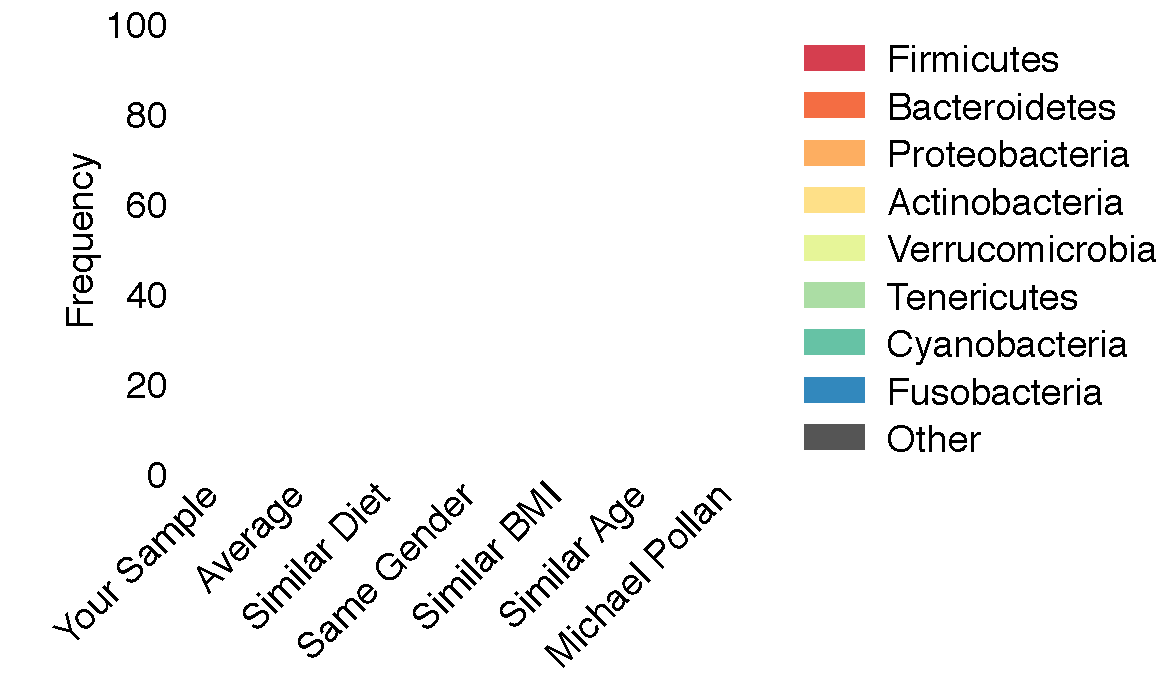
\includegraphics[width=3.65in]{pdfs-gut/figure4_overlay.pdf}}
	\end{overpic} 
    &
    {\normalsize 
    \vspace{2.5mm}
    \parbox[b][][t]{6.5in}{
	\begin{tabular}{ c l r c l r r r }
    \multicolumn{3}{l}{\large ~~Your most abundant microbes:} & \multicolumn{5}{l}{\large ~~Your most enriched microbes:}\\ \addlinespace[2mm]
        \cline{2-3} \cline{5-8} \addlinespace[1mm]
        & Taxonomy & Sample & & Taxonomy & Sample & Population & Fold \\
        \cline{2-3} \cline{5-8} \addlinespace[1mm]
        & \abundTaxonA{} & \abundSamplA{}\% & & \enrichTaxonA{} & \enrichSamplA{}\% & \enrichPopulA{}\% & \enrichFolddA{}x \\
        & \abundTaxonB{} & \abundSamplB{}\% & & \enrichTaxonB{} & \enrichSamplB{}\% & \enrichPopulB{}\% & \enrichFolddB{}x \\
        & \abundTaxonC{} & \abundSamplC{}\% & & \enrichTaxonC{} & \enrichSamplC{}\% & \enrichPopulC{}\% & \enrichFolddC{}x \\
        & \abundTaxonD{} & \abundSamplD{}\% & & \enrichTaxonD{} & \enrichSamplD{}\% & \enrichPopulD{}\% & \enrichFolddD{}x \\
        \cline{2-3} \cline{5-8} \addlinespace[3mm]
        & \multicolumn{7}{p{5.6in}}{\normalsize \rareList{}} 
	\end{tabular}
	}
	}
\end{tabular*}




\vspace{1.5cm}

{\huge How do your gut microbes compare to others?} 

\vspace{0mm}

\begin{figure}[!ht]

\hspace{11mm}
\raisebox{29mm}{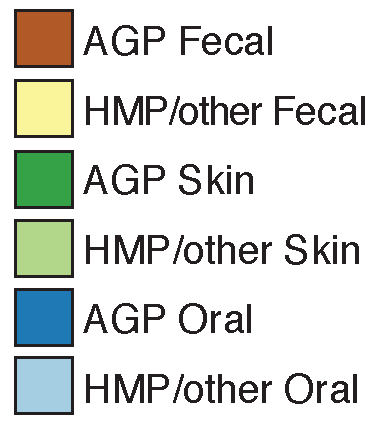
\includegraphics[scale=0.40]{pdfs-gut/figure1_legend.pdf}}
\hspace{-10mm}
\subfloat[\fontfamily{phv}\selectfont{\normalsize Different body sites}\label{subfig-1:dummy}]{%
\begin{overpic}[height=0.30\textheight]{pdfs-gut/figure1.pdf}
	\put(-2,-5){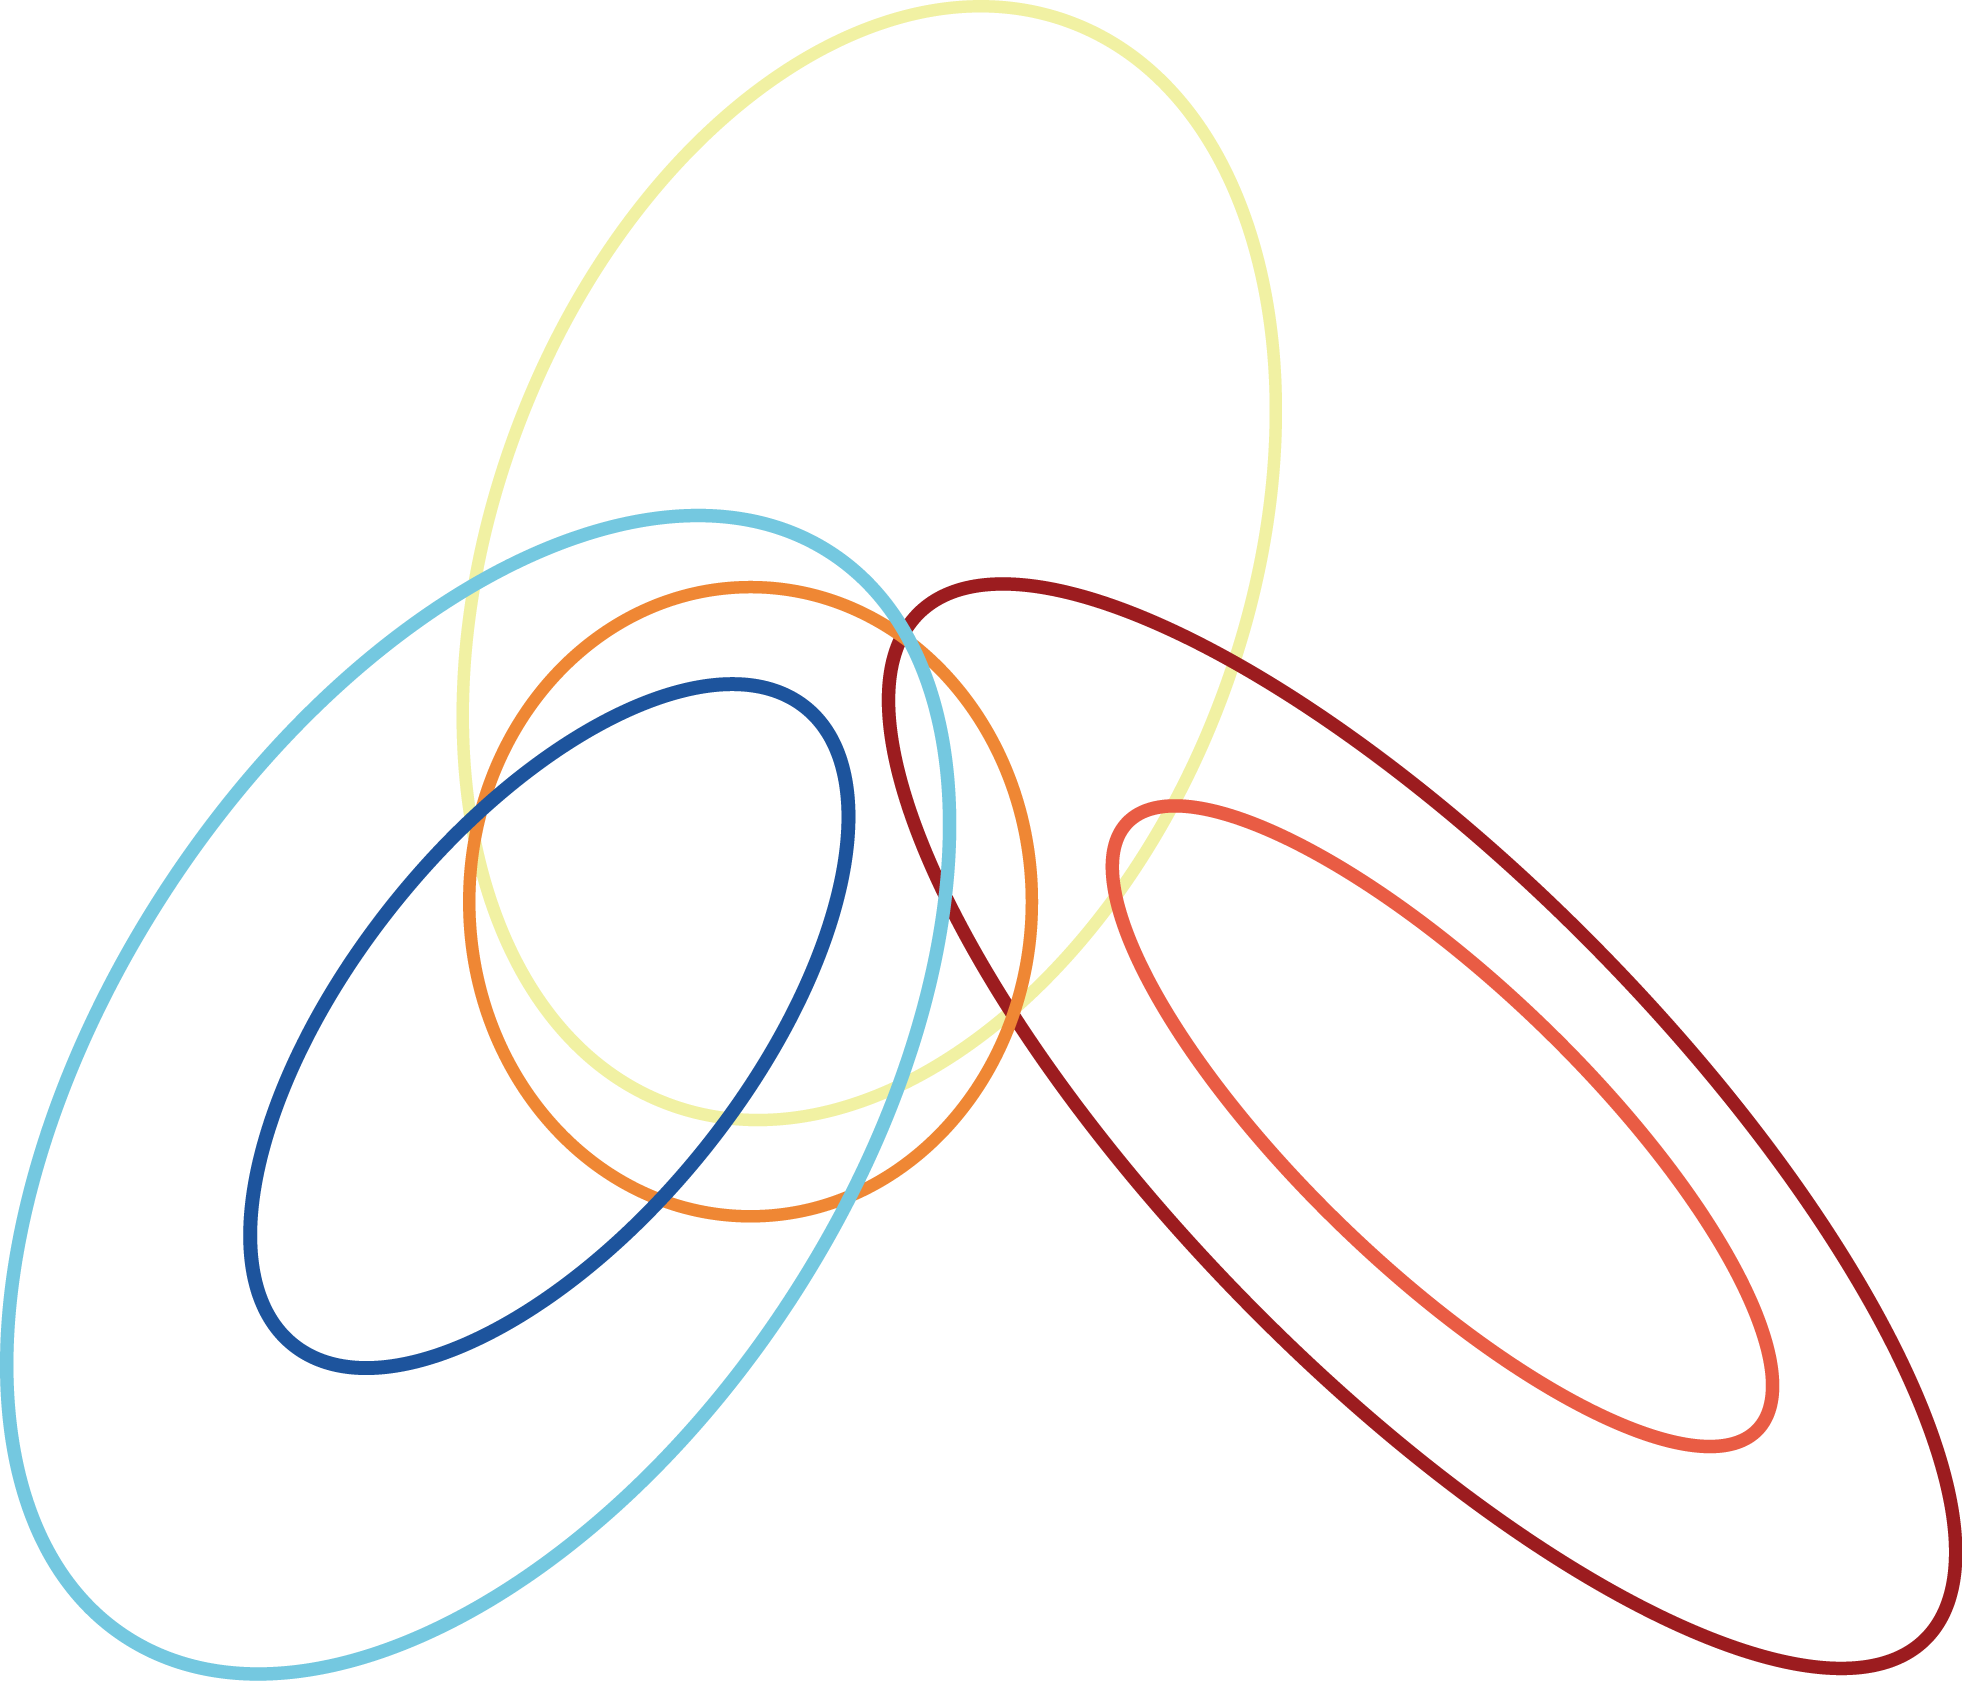
\includegraphics[scale=0.39]{pdfs-gut/figure1_ovals.png}}
\end{overpic}
}
%
\hspace{11mm}
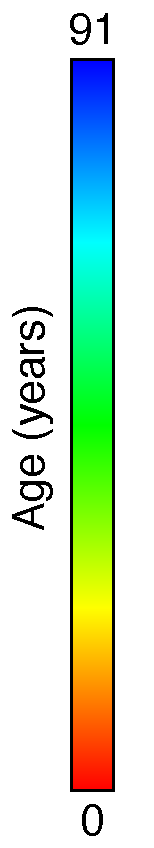
\includegraphics[scale=0.40]{pdfs-gut/figure2_legend.pdf}
\subfloat[\fontfamily{phv}\selectfont{\normalsize Different ages and populations}\label{subfig-2:dummy}]{%
\begin{overpic}[height=0.30\textheight]{pdfs-gut/figure2.pdf}
	\put(0,0){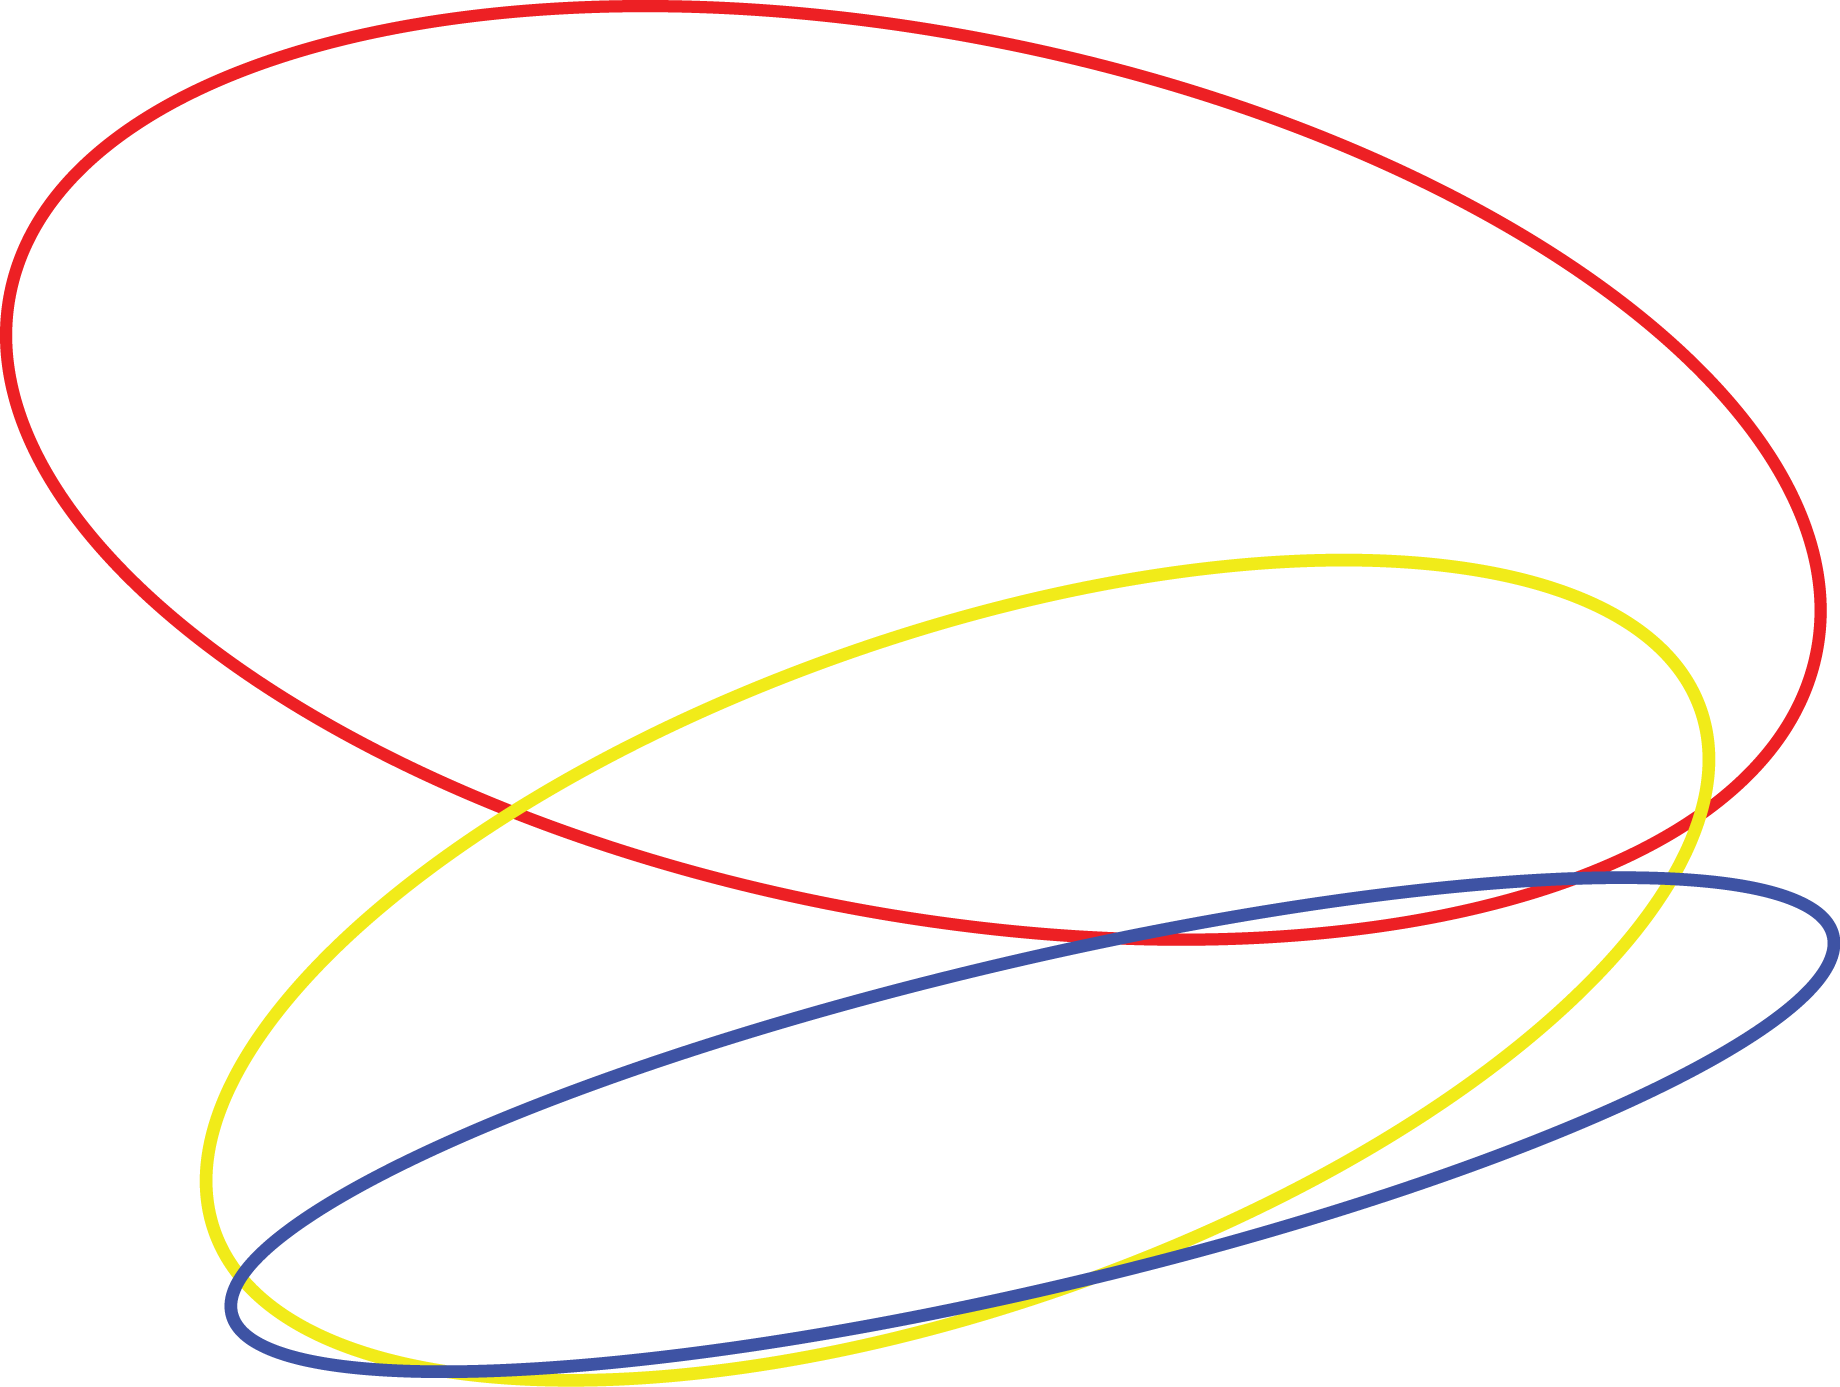
\includegraphics[scale=0.48]{pdfs-gut/figure2_ovals.png}}
	\put(180,122){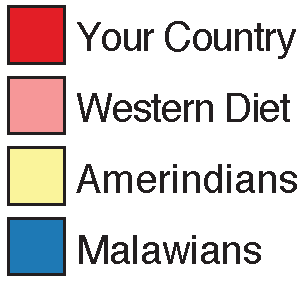
\includegraphics[scale=0.40]{pdfs-gut/figure2_country_legend.pdf}}
 	\put(130,181){
\includegraphics[scale=0.45]{pdfs-gut/ball_legend.pdf}}
\end{overpic}
}
%
\hspace{19mm}
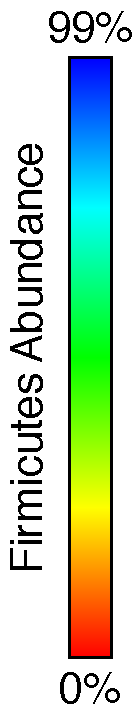
\includegraphics[scale=0.40]{pdfs-gut/figure3_legend.pdf}
\subfloat[\fontfamily{phv}\selectfont{\normalsize The American Gut population}\label{subfig-3:dummy}]{%
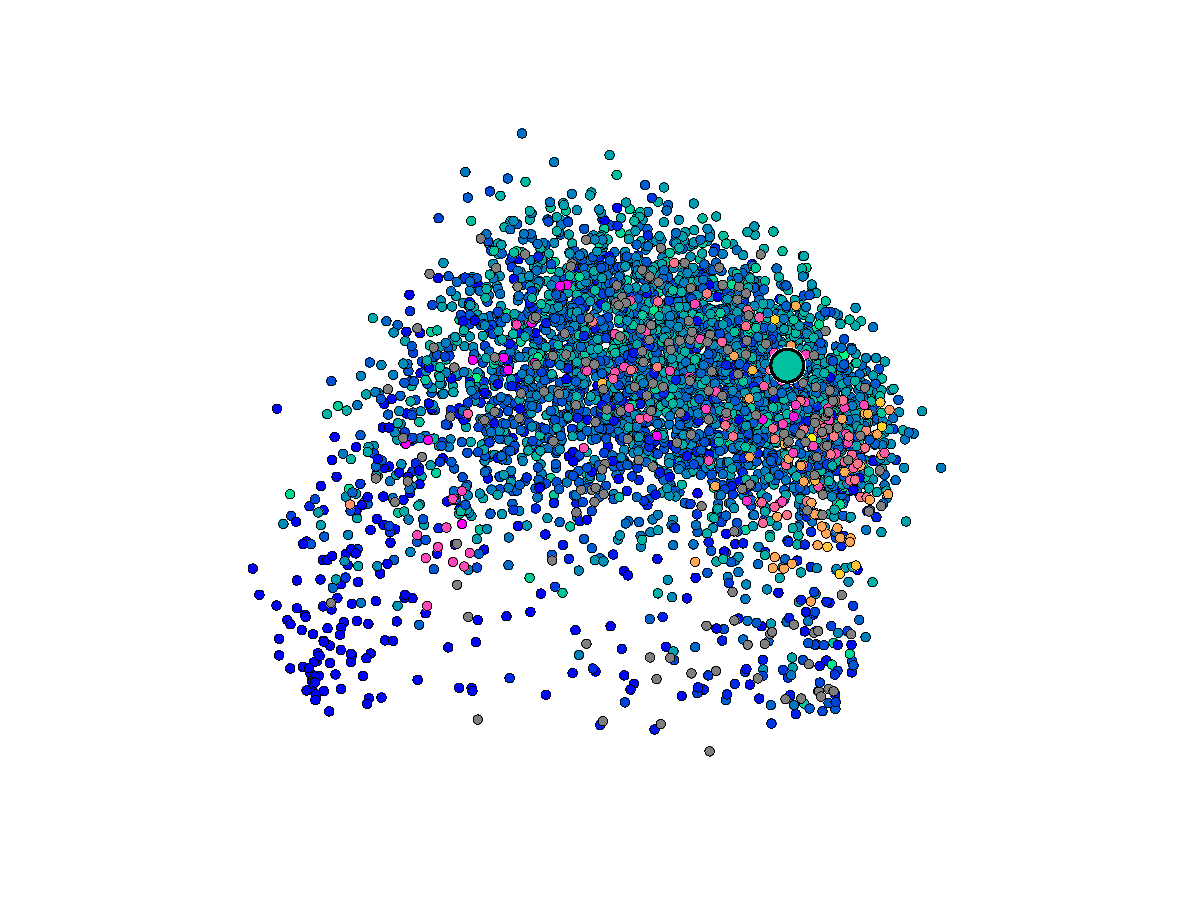
\includegraphics[height=0.30\textheight]{pdfs-gut/figure3.pdf}
}
\end{figure}



\end{document}
